\documentclass[a4paper]{article}

\usepackage{titlesec}
\usepackage{tabularx}
\usepackage{graphicx}
\graphicspath{ {./images/} }
\usepackage{pdfpages}
\usepackage[margin = 1in]{geometry}

\titleformat*{\section}{\fontsize{14}{19}\selectfont\bfseries}
\titlespacing*{\section}{0pt}{4.5ex}{1ex}

% Title Page
\title{CS344 Progress Report}
\author{Laveen Chandnani - 2004842}
\date{}

\begin{document}
	\maketitle
	\section{Overview}
	Dyck words are strings consisting of opening and closing brackets, in such a way that at any point in the string there are at least as many opening brackets as there are closing brackets on the left side of this point, and there are an equal number of opening and closing brackets in the entire string. The paper by Chistikov and Vyalyi \cite{chistikov2020re} describes a one-player game called the ``re-pairing game"; given any Dyck word, a move consists of ``pairing" an opening bracket with a closing bracket to the right of it, and erasing the two. The process is repeated until the string no longer contains any characters. Such a one-player game can have many strategies to play with, but the effectiveness of a strategy in this game is measured by it's width, which is the maximum number of nonempty segments of symbols seen during a play, and to compute the width of a Dyck word is to work out the minimum width required to re-pair the entire word.
	\newline
	\newline
	The goal of the project is to conduct a well-structured survey on the field of Dyck words and the paper by Chistikov and Vyalyi, and attempt to make progress on the first open problem at the end of the paper, which involves computing the width of a general Dyck word.
	
	\section{Progress}
	Significant progress has been made in the past 9 weeks on this project. Much of the content from Chistikov and Vyalyi's paper has been understood, with some interesting insights being made and expanded on. This is discussed further below in section 2.2.
	 
	Some algorithm design has also begun for the software to be developed over the christmas holidays; we have obtained an $O(n)$ algorithm to convert a Dyck word of length $n$ into its corresponding binary tree/forest. Although this does not directly contribute to progress on the open problem, it is interesting in its own right (and perhaps novel), and will be used when displaying the corresponding binary tree/forest for a given Dyck word in our software.
	\subsection{Objectives}
	We will be discussing the listed objectives from the updated specification (see appendix A), since the objectives in this version are more concrete.
	\begin{enumerate}
		\item An introduction to the relevant definitions and content to lay out some background knowledge.
		\item Expanding on and providing potential novel insights/perpsectives on well established results.
		\item Establishing the research landscape on the re-pairing game and relevant topics.
		\item Creating software to demonstrate re-pairing strategies from literature and allow manual experimentation on Dyck word re-pairings.
		\item Using the software to analyse subcases of Dyck words and exhaustively find their width in an attempt to pin down a formula for the width of a general Dyck word.
	\end{enumerate}
	\subsection{Objective Progress}
	\begin{enumerate}
		\item Although there is still much to be typed up in LaTeX due to this objective taking longer than expected, which is further discussed in section 3, significant progress has still been made, especially with regards to understanding the content from Chistikov and Vyalyi's paper (see appendix C for evidence of this). 
		\item There has been much progress in this area; for example a connection between Dyck words and the $n^{th}$ catalan number ($ = C_n = \frac{1}{n+1} {2n \choose n}$) has been made. This came from recognising that the restriction of there being at least as many left brackets as right brackets at any point in a Dyck word is equivalent to drawing north-east lattice walks from $(0,0)$ to $(n,n)$ but restricting the walks to have at least as many east moves as there are north moves. This meant that Dyck words correspond to north-east lattice walks that do not cross the main diagonal (the line going from $(0,0)$ to $(n,n)$), and the number of such north-east lattice walks (and subsequently, the number of Dyck words of length $2n$) is given by the $n^{th}$ catalan number. 
		
		Upon further reading, we found that the above observation is a well known one \cite{fukukawa2013counting}, but we also show that there is a 1-to-1 correspondence between Dyck words and binary forests, and so the number of binary forests that can be constructed from $n$ nodes is also given by the $n^{th}$ catalan number.
		\item No work has been done on this objective yet due to objectives 1 and 2 taking longer than expected.  Work on this objective is scheduled for the christmas holidays.
		\item Ideas have begun to develop with some progress being made towards this objective, although some issues had originally come up with using Python for the GUI as opposed to the current web-based application approach. This is discussed below in section 3. Further work on this objective is scheduled for the christmas holidays.
		\item No work on this objective can be done until the software has been developed, and so this objective has been scheduled for term 2.
	\end{enumerate}
	
	\section{Issues}
	One of the big risks from the beginning of this project has been the possibility that obtaining new findings on the open problem turns out to be infeasible. The original objectives were structured with this goal in mind, but after further effort this term it appears that making substantial progress on the open problem could very well be out of reach. As a result, the goals have been restructured to allow for a more software-oriented approach. This involves writing a program which allows us to play the re-pairing game, simulating certain strategies on Dyck words that we input into the program. The program will also allow manual re-pairing, and give the minimum width at any time during a play. We will also have a visualisation of the Dyck word as a binary tree/forest, and a visualisation of the Dyck word being re-paired, where we can step through a strategy to see how that looks on the string itself.
	
	However, the original goal of attempting to make progress on this open problem has not been abandoned, and the program will also have a brute force option, where we attempt to find the minimum width of a given Dyck word by means of an exhaustive search. This will be used to analyse subcases of Dyck words in an attempt to pin down the width of a general Dyck word.
	\newline
	\newline
	The program was originally going to be developed using the Tkinter Python library for the GUI, but after some experimentation, the library felt cumbersome to work with and had a very dated visual style and application format.
	\begin{figure}[!h]
		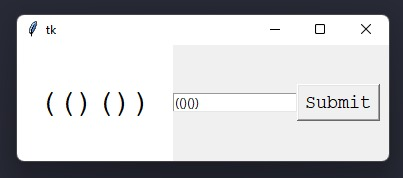
\includegraphics[width = \textwidth]{tkinter-gui.jpeg}
		\caption{Early versions of Tkinter proved to have a dated visual style}
	\end{figure}

	I am proficient in Python, and the focus of the project is on the theoretical underpinnings of re-pairing strategies, not on the implementation of the software, so using Python still seemed ideal. After some further investigation into alternatives, the conclusion was that a web-based application would be most suitable; this will allow for the backend algorithms to still be written in Python but using React and Materials UI means that the front-end is less cumbersome to work with but also has a more modern appearance. Writing the software as a web-based application also means that the software can be made accessible to other users and students regardless of the platform used.
	\newline
	\newline
	The time required to understand and digest the technical details from Chistikov and Vyalyi's paper has also taken longer than expected, meaning that we are currently behind schedule. More specifically, progress has been made on the first two objectives but has not been formally written up into LaTeX yet. However, the tasks scheduled for the christmas holidays are not expected to require the entirety of the christmas holidays, so catching up on the schedule seems feasible during this time. This will be reflected accordingly in the updated timetable below.
		
	\section{Updated Timetable}
	\begin{tabularx}{\textwidth}{|l|X|Xr}
	\hline
	\textbf{Week} & \textbf{Task} \\
	\hline
	Term 1 Week 9 & \textbf{Submission of progress report} \\
	\hline
	Term 1 Week 10 & Writing up first half of final report and begin web application implementation \\
	\hline
	w/c 12/12 & Continue writing up first half of final report and web application implementation \\
	\hline
	w/c 19/12 & Finish writing up first half of final report and continue web application implementation \\
	\hline
	w/c 26/12 & Start implementing re-pairing strategies into web application \\
	\hline
	w/c 02/01 & Finish implementing re-pairing strategies into web application and begin analysing brute force minimum widths of Dyck words \\
	\hline
	Term 2 Week 1-6 & Continue analysing results of brute force and begin writing second half of final report \\
	\hline
	Term 2 Week 7 & Begin preparation for project presentation \\ 
	\hline
	Term 2 Week 8-10 & \textbf{Project presentation} and finishing up final report \\
	\hline
	Easter Holidays & Polishing up final report \\
	\hline
	Term 3 Week 1 & \textbf{Submission of final report} \\
	\hline
	\end{tabularx}
	\newline 
	\newline
	The weekly meetings with my supervisor will also continue into term 2 to ensure the project is progressing as planned.
	
	\section{Conclusion}
	Whilst the project is currently behind schedule, the allocation of tasks for christmas holidays ensures that the impact is mitigated and the delay will not affect the outcome of the project. The work completed so far is mostly on track with the schedule, and we expect the progress to continue as such into the coming months.

	\bibliography{references}
	\bibliographystyle{ieeetr}	

%%%%%%%%%%%%%%%%%%%%%%%%%%%%%%%%%%%%%%%%%%%%%%%%%%%%%%%%%
	\newpage
	\appendix
	
	\newcommand\largesection{%
		\titleformat{\section}
		{\normalfont\huge\bfseries}{\thesection}{1em}{}
	}

	\newcommand\stdsection { %
		\titleformat{\section}
		{\normalfont\Large\bfseries}{\thesection}{1em}{}
	}
	
	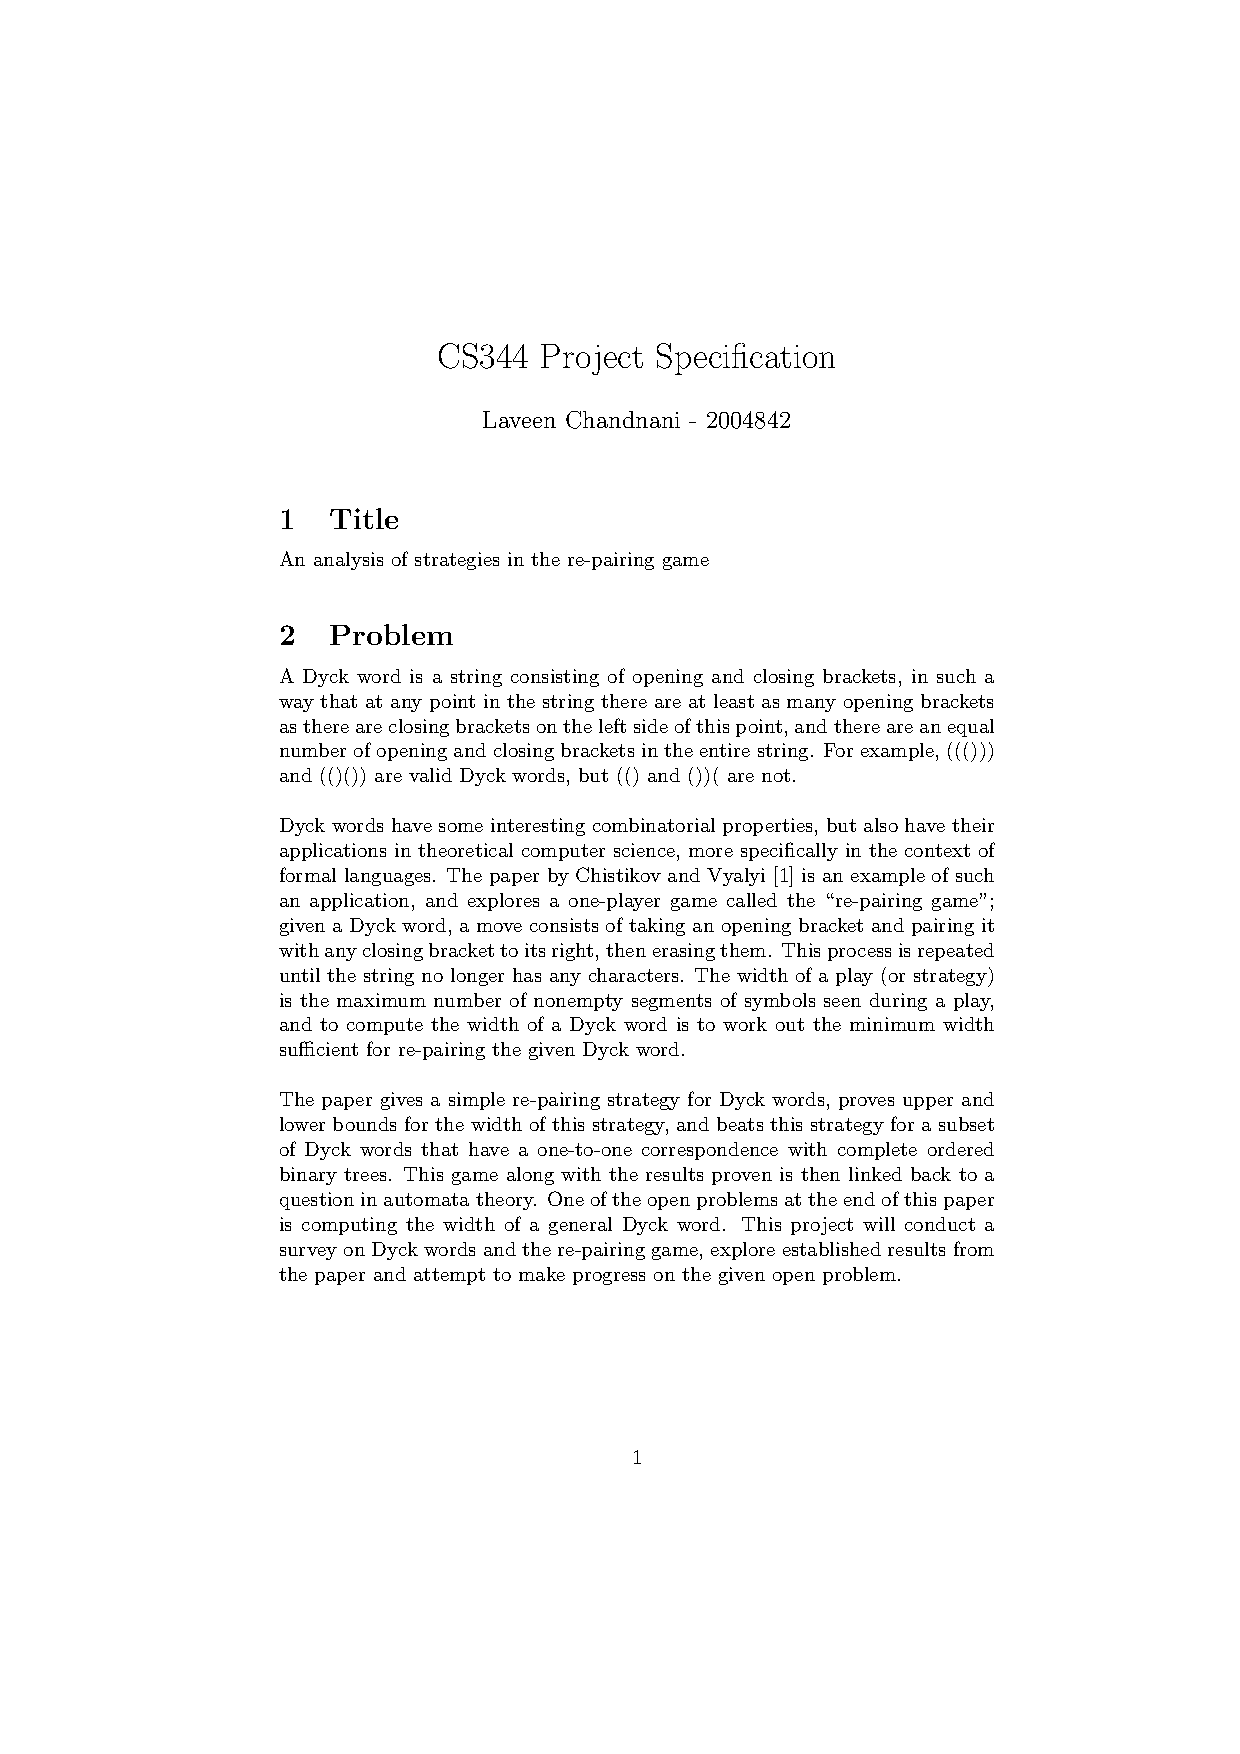
\includepdf[pages = 1, scale = 1, pagecommand = {
		\largesection
		\section*{Appendix}
		\stdsection
		\section{Up-to-date Specification}
		\label{pdf:myfile}},linktodoc = true]{./appendix-items/up-to-date-spec.pdf}
	\includepdf[pages = 2-, scale = 1, pagecommand = {}, linktodoc = true]{./appendix-items/up-to-date-spec.pdf}

	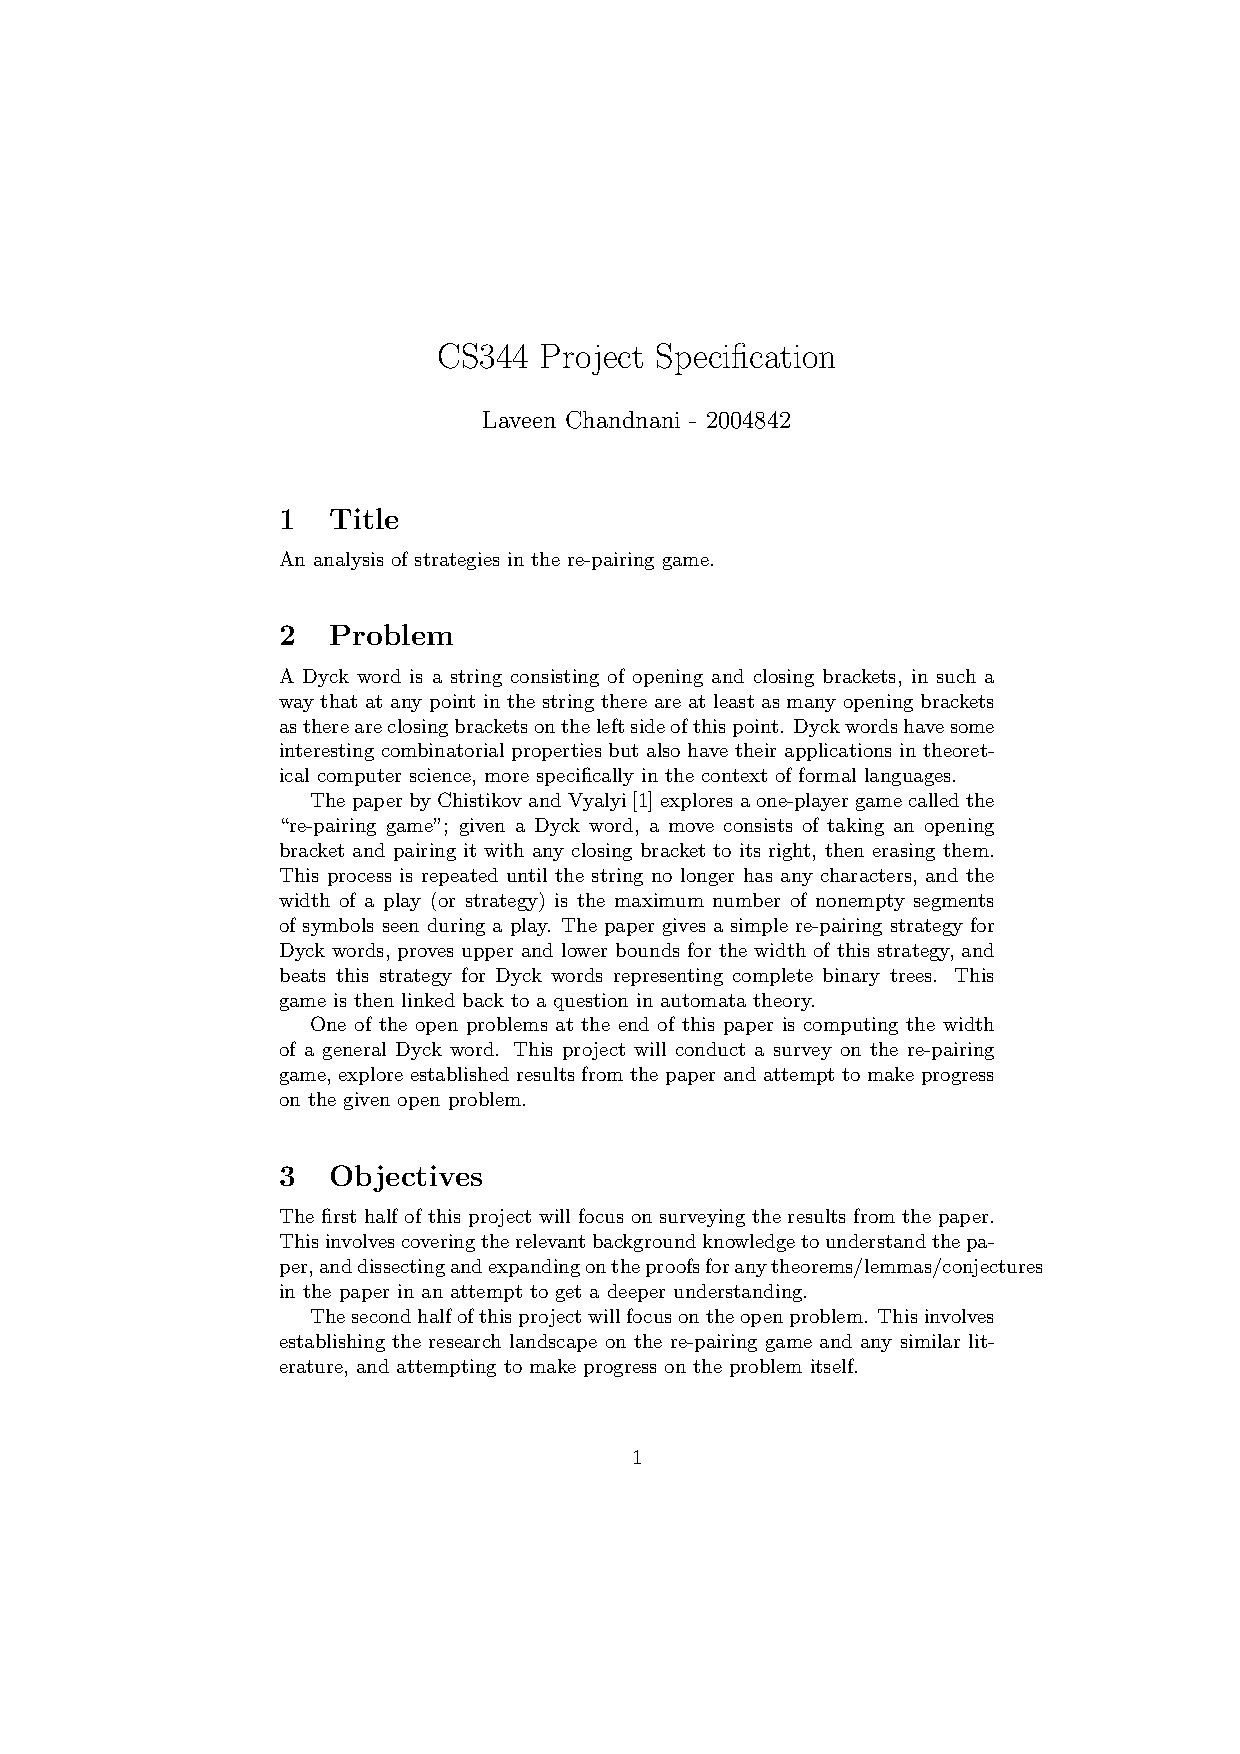
\includepdf[pages = 1,scale = 1,pagecommand = {
		\section{Original Specification}
		\label{pdf:myfile2}}, linktodoc = true]{./appendix-items/original-spec.pdf}
	\includepdf[pages = 2-, scale = 1, pagecommand = {}, linktodoc = true]{./appendix-items/original-spec.pdf}
	
	\includepdf[pages = 2, scale = .75, pagecommand = {
		\section{Evidence of work done}
		\label{pdf:myfile3}},linktodoc = true]{./appendix-items/rough-work.pdf}
	\includepdf[pages = 3-, scale = .75, pagecommand = {}, linktodoc = true]{./appendix-items/rough-work.pdf}
	
\end{document}